In questo capitolo si presenteranno i concetti e il funzionamento su cui si basa il framework Hadoop. Il capitolo si concentrerà inizialmente su una breve ricapitolazione della storia del framework, le sue origini e le cause del suo successo. Successivamente si analizzeranno nel dettaglio le sue componenti chiave ovvero HDFS e YARN e infine si introdurrà il modello Map Reduce spiegandone il funzionamento.
\section{Storia di Hadoop}
Il framework Hadoop fu creato da \textbf{Doug Cutting}, creatore di \textbf{Apache Lucene}, la libreria più utilizzata per quanto riguarda la ricerca di tipo testuale. Questo framework fonda le sue radici da \textbf{Apache Nutch}, una motore di ricerca per il web open source, a sua volta parte integrante del progetto Lucene. Scrivere un intero motore di ricerca da zero era un obiettivo molto ambizioso e il progetto Nutch partì nel 2002 ed ebbe un discreto successo tuttavia i creatori si resero immediatamente conto che la loro architettura non sarebbe stata in grado di scalare a sufficienza a causa dell'alto numero di pagine web da indicizzare (già allora ce ne erano più di un miliardo). Nel 2003 Google pubblicava il paper in cui introduceva il GFS e Nutch intuì che questo filesystem avrebbe risolto i problemi di memorizzazione e amministrazione dei dati che avevano e decisero di implementarne una versione open source che venne chiamata \textbf{NDFS} (Nutch Distributed File System). Un anno dopo Google pubblicò il paper che introdusse il paradigma Map-Reduce e ancora una volta il creatore capì che questa idea lo avrebbe aiutato a risolvere i problemi di Apache Nutch e nel 2005 il suo team implementò una sua versione open source e nel giro di 6 mesi tutti gli algoritmi del motore di ricerca furono adattati per essere eseguiti su NDFS e usando Map-Reduce. Questa "accoppiata" ebbe così tanto successo che nel Febbraio 2006, Nutch decise di spostarlo in un progetto indipendente chiamato Hadoop e nello stesso periodo Doug Cutting si unì a Yahoo! che forni un team dedicato e risorse finanziarie per trasformare Hadoop in un sistema che potesse essere eseguito per scalare anche sul web e ci riuscirono nel 2008 quando l'azienda annunciò che il suo indice di ricerca era stato generato da un cluster Hadopo da 10000 core. Nel Gennaio 2008 Hadoop divenne il progetto di punta della fondazione Apache ed è tuttora utilizzato da grandi compagnie come Facebook, New York Times e finnziato dai big dell'informatica come IBM, Microsoft e dalla stessa Google.
\section{Architettura di Hadoop}
Il passaggio dalla versione 1 alla versione 2 del framework ha portato enormi cambiamenti nella sua architettura e per evitare una descrizione troppo prolissa si introduce solamente la nuova architettura anche perchè è su quella che si basa questo lavoro. Le componenti fondamentali su cui si basa Hadoop sono le seguenti:
\begin{description}
  \item[Hadoop Common Module:] È il componente di base su cui si appoggiano tutti gli altri componenti del framework.
  \item[HDFS:] la sigla sta per "Hadoop Distributed File System" ed è il file system distribuito su cui si basa l'ecosistema Hadoop.
  \item[YARN:] Sta per "Yet Another Resource Negotiator" ed è il nuovo gestore delle risorse in Hadoop.
  \item[MapReduce:] È il componente di base che si occupa di implementare il paradigma lanciato da Google.
  \item[Altri Componenti:] Questi ultimi moduli rappresentano dei componenti che si poggiano su quelli elencati sopra.
\end{description}
\begin{figure}
  \begin{center}
    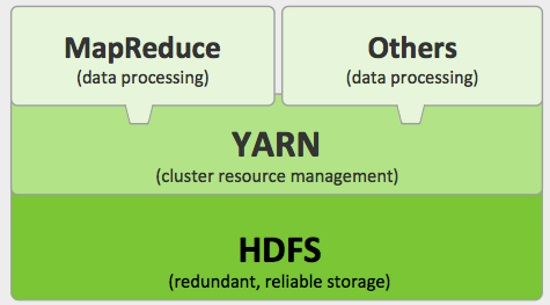
\includegraphics[width=\linewidth]{architecture.jpg}
    \caption{Architettura}
    \label{fig:architecture}
  \end{center}
\end{figure}
\subsection{HDFS}
HDFS è il filesystem distribuito che utilizza il framework Hadoop per processare i dati. I punti di forza su cui si basa sono i seguenti:
\begin{description}
  \item[Memorizzazione di grandi file:] Dove in questo contesto indichiamo file che sono centinaia di megabyte, gigabyte o terabyte.
  \item[Accesso dati:] HDFS è costruito intorno all'idea che il migiore pattern per processare i dati è "una scrittura e tante letture". Un dataset è tipicamente generato o copiato da una sorgente e successivamente varie analisi sono effettuate sul dataset nel tempo. Ogni analisi richiede grandi porzioni se non l'intero dataset quindi il tempo per leggere l'intero dataset è più importante della latenza di leggere il primo record.
  \item[Commodity Hardware:]Hadoop non richiede hardware costoso. È strutturato per essere eseguito su cluster basato su commodity hardware (hardware comunemente disponibile che può essere ottenuto da diversi fornitori).
\end{description}
\subsubsection{Blocchi}
Sappiamo che i dischi hanno una \textit{block-size} che rappresenta l'ammontare minimo di dati che possono leggere o scrivere. Di solito la grandezza di questi blocchi è nell'ordine dei kilobyte ma in HDFS questa grandezza è pari a 128MB e una caratteristica importante è che file più piccoli del blocco non occupano quest'ultimo interamente (ad esempio se avessimo un file da 1MB esso utilizzerà 1MB di disco e non 128). I motivi per cui questi blocchi sono così grandi sono vari: il primo è per minimizzare i tempi di ricerca nel disco, il secondo è che avere questa astrazione a blocchi, permette di memorizzare file più grandi di un singolo disco e inoltre semplifica la gestione della memorizzazione dei dati in quanto avere blocchi di taglia fissa permette di calcolare facilmente quanti ne possono essere memorizzati du di un disco ed elimina la gestione dei metadati (che vengono gestiti a parte).
\subsubsection{Namenode e Datanode}
Un cluster HDFS ha due tipologie di nodi che seguono il paradigma master-slave: un \textbf{namenode} (master) ed un numero di \textbf{datanode} (slave). Il primo gestisce il namespace del filesystem e i metadati per tutte le direcrory e i file e memorizza queste informazioni sul proprio disco locale oltre a conoscere la locazione dei blocchi di ogni file. I secondi invece memorizzano e processano i dati riportando periodicamente al namenode quale lista di blocchi memorizzano. La perdita del namenode comporta l'inutilizzabilità del filesystem ed è quindi importante avere un \textit{secondary-namenode} che periodicamente si sincronizza con il primary per fungere da backup in caso di guasti o malfunzionamento.
\subsection{Yarn}
\textbf{Apache YARN} (Yet Another Resource Negotiator) è il sistema della gestione delle risorse in Hadoop. Introdotto dalla versione 2 di Hadoop ha migliorato di molto le prestazioni del framework. Yarn fornisce i suoi servizi attraverso due processi manager, un \textit{resource-manager} (uno per cluster) per gestire l'uso delle risorse e un \textit{node-manager} che è eseguito su tutti i nodi nel cluster per lanciare e monitorare i container (Esegue i task con un insieme ristretto di risorse). Per eseguire un applicativo su YARN il client contatta il resource-manager e gli chiede di lanciare un \textit{application-master}. Quello che fa l'application master dipende dal tipo di applicazione: può semplicemente eseguire il job sul proprio container o richiederne altri per distribuire la computazione.
\begin{figure}
  \begin{center}
    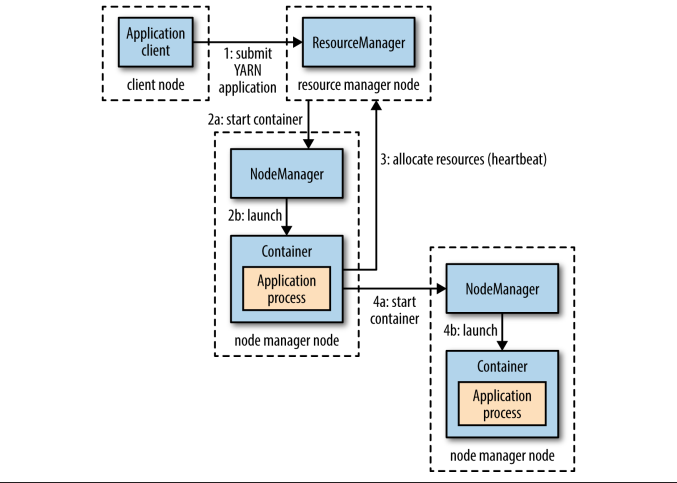
\includegraphics[width=\linewidth]{yarn.png}
    \caption{Esempio di Esecuzione di YARN}
    \label{fig:yarn}
  \end{center}
\end{figure}
\subsection{Paradigma Map-Reduce}
Map-Reduce è un modello di programmazione per processare i dati. I programmi Map-Reduce sono inerentemente paralleli, così da permettere di fare analisi di dati in larga scala se a disposizione di abbastanza macchine, in particolare questo modello funziona al meglio con dataset di grandi dimensioni. Hadoop è in grado di eseguire programmi Map-Reduce scritti in vari linguaggi tra cui Java, Python e Ruby. \\
Map-Reduce funziona suddividendo il lavoro in due fasi: la fase di map e la fase di reduce. Ogni fase ha delle coppie chiave-valore come input e output, i cui tipi potrebbero essere scelti dal programmatore. Il programmatore specifica anche due funzioni: la funzione di map e la funzione di reduce. Nello specifico Map prende in input una coppia <K,V> e restituisce in output una lista di coppie intermedie <K',V'>. Reduce prende in input una lista di coppie intermedie <K,V> con la stessa chiave e restituisce in output una lista di coppie <K',V'>. Il paradigma Map-Reduce fornisce oltre alle suddette funzioni, anche parallelizzazione e distribuzione automatica, fault tolerance, schedulazione I/O, status e monitoring. Un programma costruito secondo questo modello divide i dati in input tramite la libreria MapReduce. Vengono attivate varie istanze del programma su un cluster di macchine. Una delle istanze, il master assegna i task alle macchine, gli slave (o worker).
\subsubsection{Map}
In questa fase un worker legge il blocco di input assegnato, dopodiché estrae da esso le coppie <K,V> e le passa una alla volta alla funzione map(). La funzione map() a sua volta produce delle coppie <K',V'>.
\subsubsection{Reduce}
Il master a questo punto assegna ad un worker un task di tipo reduce indicandogli una regione di dati da "ridurre". Un task reduce consiste nel prendere tutte le coppie <K,V> raggruppate in modo che le chiavi siano uniche. Ogni gruppo viene passato quindi alla funzione reduce().
\subsubsection{Splitter}
Lo Splitter è quella componente che ha il compito di prendere l’intero input e di dividerlo in InputSplits, che verranno poi inviati ai vari map task. La mappatura < K, V > degli InputSplits viene definita dalla classe InputFormats implementata. Hadoop mette a disposizione diverse implementazioni di InputFormat, ciononostante è possibile, ovviamente, definire un proprio InputFormat da utilizzare durante la computazione implementando l’interfaccia InputFormat. \\
È da sottolineare il fatto che non si deve confondere l’InputSplit con il blocco utilizzato dall’HDFS. I due ”blocchi” non necessariamente corrispondono. Possono infatti verificarsi dei casi in cui l’InputSplit utilizza dati presenti in più blocchi, causando un leggero overhead del sistema.
\subsubsection{Partitioner}
I Partitioners sono responsabili di dividere le coppie < K, V > intermedie generate dai MapTasks ai vari Reducers per la funzione di Reduce. Per dividere in maniera equa i compiti ai Reducers i partitioners usano una funzione di hash sulla chiave: reducer = hash(K) mod n.
\subsubsection{Combiner}
I Combiners permettono l'aggregazione in locale prima della fasi di shuffle e sorting.
\subsubsection{Shuffle e Sort}
Map-Reduce garantisce che l'input ad ogni reducer sia ordinato per chiave. Il processo con il quale il sistema esegue il sort, e trasferisce gli output del map ai reducer come input, è conosciuto come shuffle.
\section{Come funziona un Job Map Reduce}
A grandi linee possiamo riassumere un'esecuzione di MapReduce nei seguenti punti:
\begin{enumerate}
  \item lettura dei dati;
  \item inputsplitting;
  \item mapping;
  \item combining; al metodo 
  \item partitioning, shuffling e sorting;
  \item reducing.
\end{enumerate}
È possibile eseguire un job MapReduce con una singola chiamata al metodo submit() di un oggetto Job. Questa chiamata al metodo cela molta computazione ed è opportuno capire quali sono i passi compiuti da Hadoop  per eseguire un job. \\
L'intero processo comprende, da una vista ad alto livello, cinque entità indipendenti:
\begin{enumerate}
  \item il client, che sottomette il job MapReduce;
  \item il resource maanger YARN, che coordina e monitora i container di calcolo sulle macchine del cluster;
  \item i node manager YARN, che lanciano e monitorano i container di calcolo sulle macchine del cluster;
  \item l'application master MapReduce, che coordina i task che eseguono il job MapReduce. L'application master e i task MapReduce sono eseguiti in container che sono schedulati dal resource manager e gestiti dai node manager;
  \item il distributed filesystem (HDFS), che è usato per condivedere file tra altre entità.
\end{enumerate}
\begin{figure}
  \begin{center}
    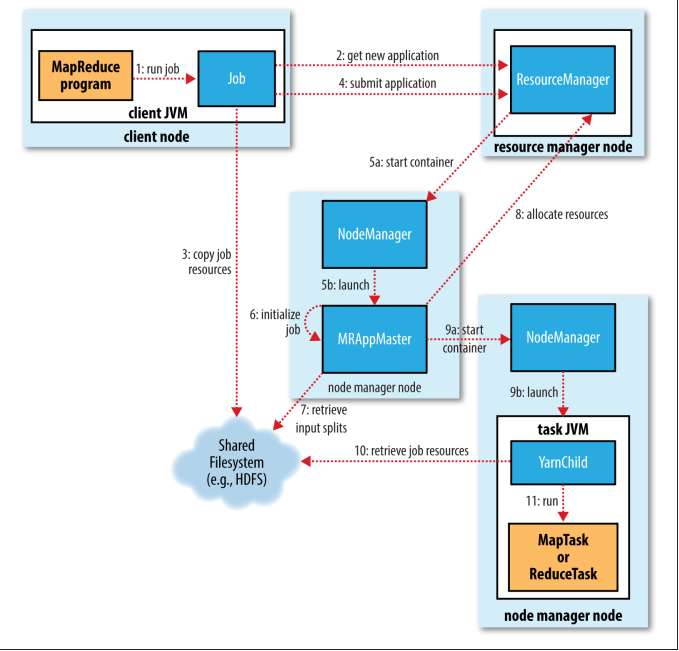
\includegraphics[width=\linewidth]{mapReduceJob.png}
    \caption{L'esecuzione di un job MapReduce di Hadoop}
    \label{fig:job}
  \end{center}
\end{figure}
\subsection{Sottomissione del Job}
Il metodo submit() effettuato su un Job crea un'istanza interna JobSubmitter e chiama submitJobInterval() su di esso. Avendo sottomesso il job, waitForCompletion() sonda il progresso di job e riporta il progresso alla console se è cambiato dall'utlimo report. Quando un job è completato con successo, il job sono counter sono mostatrati. Altrimenti, l'errore che ha causato il fail del job è loggato in console.
\subsection{Inizializzazione del job}
Quando il resource maanger riceve una chiamata al suo metodo submitApplication(), consegna la richiesta allo YARN scheduler. Lo scheduler alloca un container, e il resource manager quindi lancia il processo dell'application master qui, sotto la gestione del node manager. \\
L'application master per i job MapReduce è un'applicazione Java la cui main class è MRAppMaster. Esso inizializza il job creando un numero di oggetti bookkeping per tenere traccia del progresso del job, dato che riceverà report sul progresso e sul completamento dai task. Successivamente, recupera gli input split calcolati nel client dal filesystem condiviso. Quindi crea un oggetto map task per ogni split, così come un numero di oggetti reduce task determinato dalla proprietà mapreduce,.job.reduces. I task a questo punto ricevono l'ID. \\
L'application master deve decidere come eseguire i task che costituiscono il job MapReduce. Se il job è piccolo, l'application master potrebbe scegliere di eseguire i task nella sua stessa JVM. \\
Infine, prima che qualsiasi task venga eseguito, l'application master chiama il metodo setupJob() sull'OutputCommitter. Per il FileOutputCommitter, che è di default, creerà la directory di output finale per il job e lo spazio di lavoro temporaneo per il task di output.
\subsection{Esecuzione del Task}
Una volta che a un task sono state assegnate risorse per un container su un particolare nodo dallo scheduler del resource manager, l'application master avvia il container contattando il node manager. Il task è eseguito da un'applicazione Java la cui main class è YarnChild. Prima che possa eseguire il task, localizza le risorse di cui il task ha bisogno, inclusa la configurazione del job e un JAR file, e qualsiasi file dalla cache distribuita. Alla fine, esegue il map o il reduce task. \\
Il YarnChild è eseguito in una JVM dedicata, così che qualsiasi bug nel map user-defined e le funzioni reduce (o anche in YarnChild) non influenzino il node manager, causandone il crash. \\
Ogni task può eseguire azioni di setup e commit, che sono eseguite sulla stessa JVM come il task stesso e sono determinate dall'OutputCommitter per il job. Per i job file-based, il commit sposta l'output del task da una locazione temporanea alla sua locazione finale. Il protocollo di commit assicura che quando l'esecuzione speculativa è abilitata, solo di uno dei task duplicati verrà fatto il commit e gli altri saranno abortiti.
\subsection{Completamento di un job}
Quando il master application riceve una notifica che l'ultimo task per un job è completo, cambia lo stato per il job a "successful". Quindi, quando il Job sonda lo stato, apprende che il job è stato completato con successo, quindi stampa un messaggio per dirlo all'utente e quindi ritorna dal metodo waitForCompletion(). Le statistiche e i counter di un Job sono stampati su console a questo punto. \\
L'application master invia anche una job notification HTTP se è configurato per farlo. Questo può essere configurato dai client che vogliono ricevere callback, tramite la proprietà mapreduce.job.end-notification.url. \\
Infine, al completamento di un job, l'application master e i task container puliscono il loro working state (così l'output intermedio è cancellato), e il metodo commitJob() di OutputCommitter è chiamato. Informazioni del Job sono registrate dal job history erver per consentire successive interrogazioni dagli utenti se desiderato.
\subsection{Shuffle e Sort}
Lo shuffle è un'area del codebase dove raffinamenti e miglioramenti sono continuamente effettuati, costituisce il cuore di MapReduce ed è qui che avviene la "magia".
\subsubsection{Il lato Map}
Quando la funzione map comincia a produrre output, non è semplicemente scritto su disco. Il processo è più complesso, e prende vantaggi dalla bufferizzazione delle scritture in memoria ed fa quale preordinamento per ragioni di efficienza. \\
Ogni map task ha un buffer di memoria circolare su cui scrive l'output. Quando i contenuti del buffer raggiungono un certo limite di taglia, un thread in background comincerà a SPILL scrivere i contenuti su disco. I map output continueranno a essere scritti sul buffer fino a quando la scrittura


















